\documentclass{standalone}
\usepackage{tikz}
\usetikzlibrary{patterns, positioning}

\begin{document}
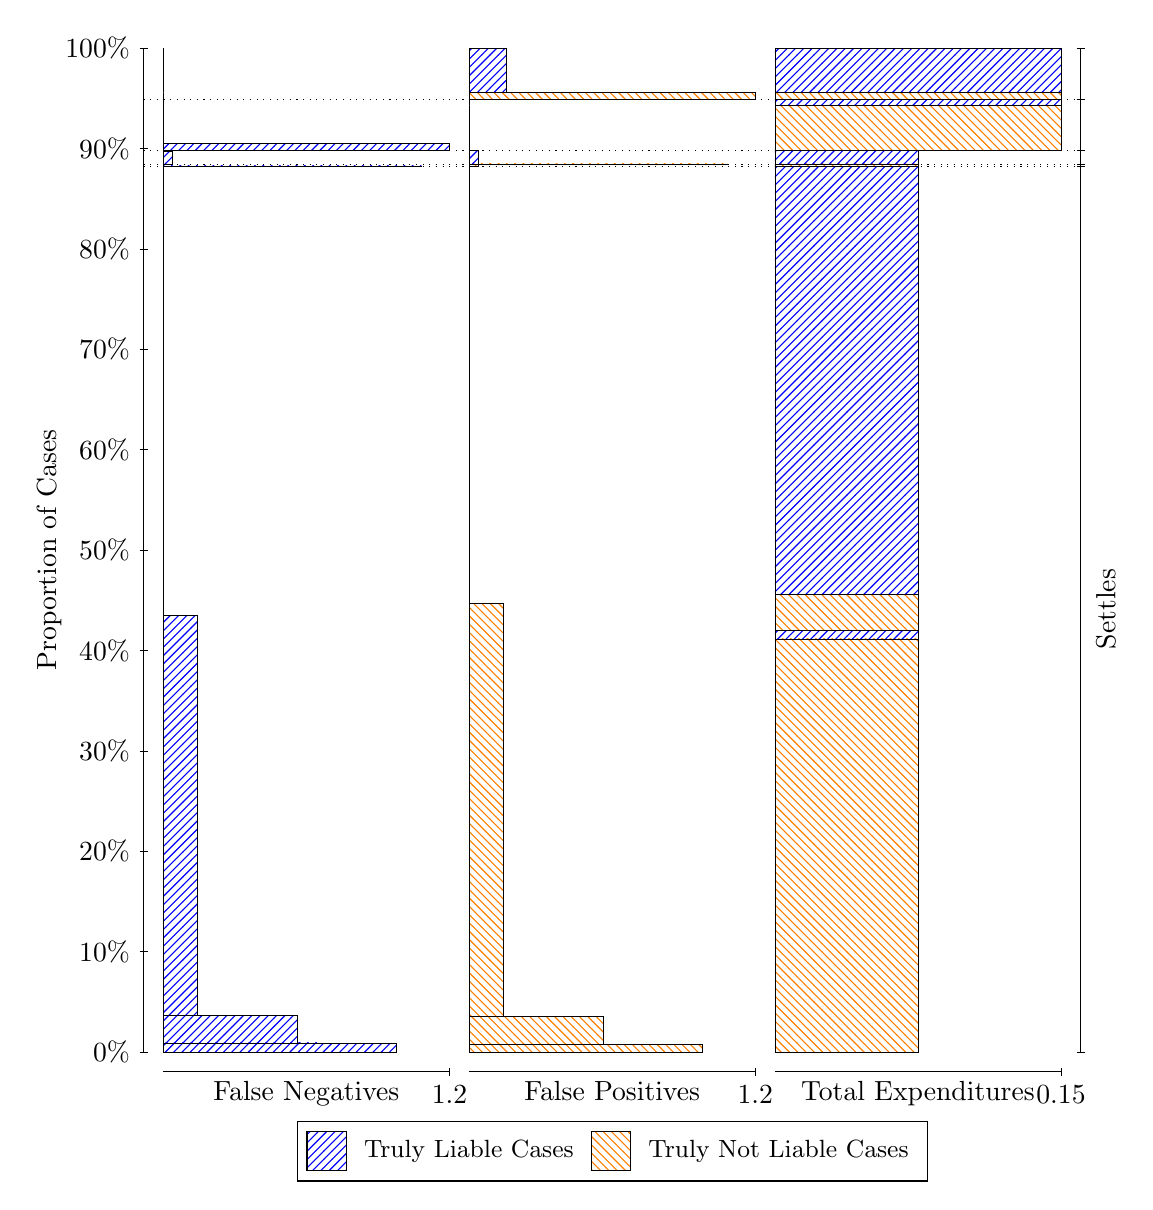
\begin{tikzpicture}
\draw[black, very thin] (1.5,1.75) -- (1.5,14.5);
\node[rotate=90, anchor=center] at (0.3, 8.125) {Proportion of Cases};
\draw[black, very thin] (1.45,1.75) -- (1.55,1.75);
\node[anchor=east] at (1.45, 1.75) {0\%};
\draw[black, very thin] (1.45,3.025) -- (1.55,3.025);
\node[anchor=east] at (1.45, 3.025) {10\%};
\draw[black, very thin] (1.45,4.3) -- (1.55,4.3);
\node[anchor=east] at (1.45, 4.3) {20\%};
\draw[black, very thin] (1.45,5.575) -- (1.55,5.575);
\node[anchor=east] at (1.45, 5.575) {30\%};
\draw[black, very thin] (1.45,6.85) -- (1.55,6.85);
\node[anchor=east] at (1.45, 6.85) {40\%};
\draw[black, very thin] (1.45,8.125) -- (1.55,8.125);
\node[anchor=east] at (1.45, 8.125) {50\%};
\draw[black, very thin] (1.45,9.4) -- (1.55,9.4);
\node[anchor=east] at (1.45, 9.4) {60\%};
\draw[black, very thin] (1.45,10.675) -- (1.55,10.675);
\node[anchor=east] at (1.45, 10.675) {70\%};
\draw[black, very thin] (1.45,11.95) -- (1.55,11.95);
\node[anchor=east] at (1.45, 11.95) {80\%};
\draw[black, very thin] (1.45,13.225) -- (1.55,13.225);
\node[anchor=east] at (1.45, 13.225) {90\%};
\draw[black, very thin] (1.45,14.5) -- (1.55,14.5);
\node[anchor=east] at (1.45, 14.5) {100\%};

\draw[black, very thin] (13.4,1.75) -- (13.4,14.5);
\draw[black, very thin] (13.35,1.75) -- (13.45,1.75);
\node[anchor=west] at (13.35, 1.75) {};
\draw[black, very thin] (13.35,12.999) -- (13.45,12.999);
\node[anchor=west] at (13.35, 12.999) {};
\draw[black, very thin] (13.35,13.023) -- (13.45,13.023);
\node[anchor=west] at (13.35, 13.023) {};
\draw[black, very thin] (13.35,13.203) -- (13.45,13.203);
\node[anchor=west] at (13.35, 13.203) {};
\draw[black, very thin] (13.35,13.851) -- (13.45,13.851);
\node[anchor=west] at (13.35, 13.851) {};
\draw[black, very thin] (13.35,14.5) -- (13.45,14.5);
\node[anchor=west] at (13.35, 14.5) {};

\draw[black, very thin, pattern color=blue, pattern=north east lines] (1.75,1.75) rectangle (4.712,1.8575);
\draw[black, very thin, pattern color=blue, pattern=north east lines] (1.75,1.8575) rectangle (4.396,1.8605);
\draw[black, very thin, pattern color=blue, pattern=north east lines] (1.75,1.8605) rectangle (4.0801,1.8635);
\draw[black, very thin, pattern color=blue, pattern=north east lines] (1.75,1.8635) rectangle (3.7641,1.8666);
\draw[black, very thin, pattern color=blue, pattern=north east lines] (1.75,1.8666) rectangle (3.4482,2.2123);
\draw[black, very thin, pattern color=blue, pattern=north east lines] (1.75,2.2123) rectangle (2.1844,7.2994);
\draw[black, very thin, pattern color=orange, pattern=north west lines] (1.75,7.2994) rectangle (1.75,12.999);
\draw[black, very thin, pattern color=blue, pattern=north east lines] (1.75,12.999) rectangle (5.0279,13.003);
\draw[black, very thin, pattern color=orange, pattern=north west lines] (1.75,13.003) rectangle (1.75,13.023);
\draw[black, very thin, pattern color=blue, pattern=north east lines] (1.75,13.023) rectangle (1.8685,13.195);
\draw[black, very thin, pattern color=orange, pattern=north west lines] (1.75,13.195) rectangle (1.75,13.203);
\draw[black, very thin, pattern color=blue, pattern=north east lines] (1.75,13.203) rectangle (5.3833,13.286);
\draw[black, very thin, pattern color=orange, pattern=north west lines] (1.75,13.286) rectangle (1.75,13.851);
\draw[black, very thin, pattern color=orange, pattern=north west lines] (1.75,13.851) rectangle (1.75,13.934);
\draw[black, very thin, pattern color=blue, pattern=north east lines] (1.75,13.934) rectangle (1.75,14.5);
\draw[black, very thin, pattern color=orange, pattern=north west lines] (5.6333,1.75) rectangle (8.5953,1.8507);
\draw[black, very thin, pattern color=orange, pattern=north west lines] (5.6333,1.8507) rectangle (7.3315,2.1984);
\draw[black, very thin, pattern color=orange, pattern=north west lines] (5.6333,2.1984) rectangle (7.0156,2.2007);
\draw[black, very thin, pattern color=orange, pattern=north west lines] (5.6333,2.2007) rectangle (6.6996,2.2029);
\draw[black, very thin, pattern color=orange, pattern=north west lines] (5.6333,2.2029) rectangle (6.3837,2.2052);
\draw[black, very thin, pattern color=orange, pattern=north west lines] (5.6333,2.2052) rectangle (6.0678,7.4497);
\draw[black, very thin, pattern color=blue, pattern=north east lines] (5.6333,7.4497) rectangle (5.6333,12.999);
\draw[black, very thin, pattern color=orange, pattern=north west lines] (5.6333,12.999) rectangle (5.7518,13.019);
\draw[black, very thin, pattern color=blue, pattern=north east lines] (5.6333,13.019) rectangle (5.6333,13.023);
\draw[black, very thin, pattern color=orange, pattern=north west lines] (5.6333,13.023) rectangle (8.9112,13.03);
\draw[black, very thin, pattern color=blue, pattern=north east lines] (5.6333,13.03) rectangle (5.7518,13.203);
\draw[black, very thin, pattern color=orange, pattern=north west lines] (5.6333,13.203) rectangle (5.6333,13.768);
\draw[black, very thin, pattern color=blue, pattern=north east lines] (5.6333,13.768) rectangle (5.6333,13.851);
\draw[black, very thin, pattern color=orange, pattern=north west lines] (5.6333,13.851) rectangle (9.2667,13.934);
\draw[black, very thin, pattern color=blue, pattern=north east lines] (5.6333,13.934) rectangle (6.1072,14.5);
\draw[black, very thin, pattern color=orange, pattern=north west lines] (9.5167,1.75) rectangle (11.333,6.9967);
\draw[black, very thin, pattern color=blue, pattern=north east lines] (9.5167,6.9967) rectangle (11.333,7.1072);
\draw[black, very thin, pattern color=orange, pattern=north west lines] (9.5167,7.1072) rectangle (11.333,7.5602);
\draw[black, very thin, pattern color=blue, pattern=north east lines] (9.5167,7.5602) rectangle (11.333,12.999);
\draw[black, very thin, pattern color=orange, pattern=north west lines] (9.5167,12.999) rectangle (11.333,13.019);
\draw[black, very thin, pattern color=blue, pattern=north east lines] (9.5167,13.019) rectangle (11.333,13.023);
\draw[black, very thin, pattern color=orange, pattern=north west lines] (9.5167,13.023) rectangle (11.333,13.03);
\draw[black, very thin, pattern color=blue, pattern=north east lines] (9.5167,13.03) rectangle (11.333,13.203);
\draw[black, very thin, pattern color=orange, pattern=north west lines] (9.5167,13.203) rectangle (13.15,13.768);
\draw[black, very thin, pattern color=blue, pattern=north east lines] (9.5167,13.768) rectangle (13.15,13.851);
\draw[black, very thin, pattern color=orange, pattern=north west lines] (9.5167,13.851) rectangle (13.15,13.934);
\draw[black, very thin, pattern color=blue, pattern=north east lines] (9.5167,13.934) rectangle (13.15,14.5);
\draw[black, dotted] (1.5,12.999) -- (13.4,12.999);
\draw[black, dotted] (1.5,13.023) -- (13.4,13.023);
\draw[black, dotted] (1.5,13.203) -- (13.4,13.203);
\draw[black, dotted] (1.5,13.851) -- (13.4,13.851);
\draw[black, very thin] (1.75,1.5) -- (5.3833,1.5);
\node[anchor=north] at (3.5667, 1.5) {False Negatives};
\draw[black, very thin] (5.3833,1.45) -- (5.3833,1.55);
\node[anchor=north] at (5.3833, 1.45) {1.2};

\draw[black, very thin] (5.6333,1.5) -- (9.2667,1.5);
\node[anchor=north] at (7.45, 1.5) {False Positives};
\draw[black, very thin] (9.2667,1.45) -- (9.2667,1.55);
\node[anchor=north] at (9.2667, 1.45) {1.2};

\draw[black, very thin] (9.5167,1.5) -- (13.15,1.5);
\node[anchor=north] at (11.333, 1.5) {Total Expenditures};
\draw[black, very thin] (13.15,1.45) -- (13.15,1.55);
\node[anchor=north] at (13.15, 1.45) {0.15};

\node[black, centered, rotate=90] at (13.72, 7.3745) {Settles};





\draw (7.449999999999999,1.5) node[draw=none] (baseCoordinate) {};
\begin{scope}[align=center]
        \matrix[scale=0.5, draw=black, below=0.5cm of baseCoordinate, nodes={draw}, column sep=0.1cm]{
            \node[rectangle, draw, minimum width=0.5cm, minimum height=0.5cm, pattern=north east lines, pattern color=blue] {}; &
            \node[draw=none, font=\small] (B) {Truly Liable Cases}; &
            \node[rectangle, draw, minimum width=0.5cm, minimum height=0.5cm, pattern=north west lines, pattern color=orange] {}; &
            \node[draw=none, font=\small] (B) {Truly Not Liable Cases}; \\
            };
\end{scope}

\end{tikzpicture}
\end{document}